\documentclass[12pt]{article}
\usepackage{graphicx}
\usepackage{amsmath}
\usepackage{parskip}
\usepackage[utf8]{inputenc}
\usepackage[T1]{fontenc}
\usepackage{lmodern}
\usepackage{color}
\usepackage{hyperref}
\usepackage{amsmath}
\usepackage{amsfonts}
\usepackage[table]{xcolor}
\usepackage{float}
\usepackage[framed, numbered]{mcode}
\usepackage[margin=3cm]{geometry}
\usepackage{subfig}
\usepackage[numbers]{natbib}

\hypersetup{
        hidelinks
}

\lstset{basicstyle=\fontsize{9}{12}\ttfamily}

\begin{document}

\title{Machine Learning in Network Biology\\Homework 1}
\author{
    Dr. Amin Emad \\ \\
    Gian Favero: 261157396 \\
}
\date{October 6th, 2023}
\maketitle
\newpage

% \tableofcontents
% \newpage

\section{Introduction}
Transcriptomic data refers to a collection of RNA molecules, or transcripts, present in cell tissues at a reference time. Typically, these molecules are generated in a cell through the process of transcription of DNA into RNA. This data contains insights into the expression levels of genes in a cell which can be used to predict various items like disease, stimuli response, and development, among others \cite{noauthor_transcriptome_nodate}.

Several classical machine learning approaches can be used when analyzing transcriptomic data. These include dimensionality reduction, clustering, and regression. All three of these particular approaches will be explored in this assignment using popular Python libraries to gain some insight into the data provided. Gene expression data was provided alongside this assignment(\verb|gdsc_expr_postCB.csv|) and drug response data (\verb|gdsc_dr.csv|). The file contains rows that begin with a gene name and are taken to be features of the data, while columns represent gene lines, or instances. 

\section{Part 1: Dimensionality Reduction}
Dimensionality reduction is a technique used to reduce the number of features in a dataset. This is done by projecting the data onto a lower dimensional space and finding a new, simpler set of features that can be used to represent the original data. Memory usage, computational efficiency, and visualization are all advantages of dimensionality reduction.

Several dimensionality reduction techniques are explored in this assignment. These include Principal Component Analysis (PCA), UMAP, and t-SNE algorithms.

\subsection{Theory}
\subsubsection{Principal Component Analysis}
The following is adapted from Goodfellow et al. \cite{GoodBengCour16}.

For a set of \textit{m} data points $\textbf{x}^{(i)}$ $\in$ $\mathbb{R}^n$, PCA finds a lower dimensional representation of the data by representing it as a code vector $\textbf{c}^{(i)}$ $\in$ $\mathbb{R}^l$ where $l < n$. The goal of PCA is to find a function $f$ such that $\textbf{c}^{(i)}$ = $f(\textbf{x}^{(i)})$ and a decoding function $g$ which provides $\textbf{x} \approx g(f(\textbf{x}))$. This is simply done using a decoding matrix, $\textbf{D} \in \mathbb{R}^{n \times l}$ which has columns that are orthogonal and have a unit norm. Following this, the code vector is given by:
\begin{align*}
    \textbf{c} = f(\textbf{x}) = \textbf{D}^T\textbf{x}
\end{align*}
and the reconstructed input is given by:
\begin{align*}
    \textbf{x} \approx g(\textbf{c}) = \textbf{D}\textbf{D}^T\textbf{x}
\end{align*} 

Using a closed-form or numerical optimization method, the decoding matrix can be found by minimizing the reconstruction error, $||\textbf{x} - \textbf{D}\textbf{D}^T\textbf{x}||_2^2$ across each point in the dataset.
 
$l$ is typically the only parameter selected by the user. For visual purposes, $l$ is typically chosen as 2 such that the compressed data can be plotted on a Cartesian plane.

\subsubsection{t-SNE}
t-SNE was proposed by Van der Maaten et al. \cite{vanDerMaaten2008} as a technique for visualizing high-dimensional data. At a high-level, the algorithm maps each data point to a location on a 2D or 3D map that can reveal the structure at many scales. The resulting map effectively reveals low-dimensional manifolds on which the data points lie.

t-SNE algorithms are incorporated into the \verb|scikit-learn| Python library. The algorithm is capable of optimizing a dimensionality reduction on a dataset based on a number of parameters selected by a user. Some of these include the number of dimensions and the perplexity, which dictate the manner in which the algorithm structures the lower-dimension manifolds in which the data lies.

\subsubsection{UMAP}
UMAP is a novel non-linear manifold learning technique by McInnes et al. \cite{mcinnes_umap_2020}. UMAP is a scalable algorithm that is comparable to t-SNE in visualization, but superior in runtime and preservation of global structure.

UMAP algorithms have been abstracted into a Python library, \verb|umap-learn|, which is capable of optimizing a dimensionality reduction on a dataset based on a number of parameters selected by a user. Some of these include the number of dimensions, the number of neighbors and the minimum distance between points, which play roles in the generalization of the algorithm, the trends identified (local or global), and the distinction between clusters.

\subsection{Implementation}
Brief data pre-processing was done before implementing the different dimensionality reduction techniques. Commonly used libraries such as \verb|numpy| and \verb|matplotlib| were imported, before the data was loaded into a numpy array, stripped of its first row (instance headers) and its first column (feature headers) and transposed such that the data was in the form of a $n \times m$ matrix where $n$ is the number of instances and $m$ is the number of features.

The dimensionality reduction techniques were then implemented. The \verb|scikit-learn| library was used to implement PCA and t-SNE, while the \verb|umap-learn| library was used to implement UMAP. Specifically, the \verb|sklearn.decomposition.PCA|, \verb|umap|, and \verb|sklearn.manifold| classes were used for \href{https://scikit-learn.org/stable/modules/generated/sklearn.decomposition.PCA.html}{PCA}, \href{https://umap-learn.readthedocs.io/en/latest/parameters.html}{UMAP}, and \href{https://scikit-learn.org/stable/modules/generated/sklearn.manifold.TSNE.html}{t-SNE} respectively. Please refer to the linked documentation for more information on the class parameters and their default values.

First, the techniques were implemented with their default parameters with the exception of the number of dimensions, which was set to 2 for all techniques. The results of this implementation are shown in Figure \ref{fig:default_dimred}.

\begin{figure}[H]
    \centering
    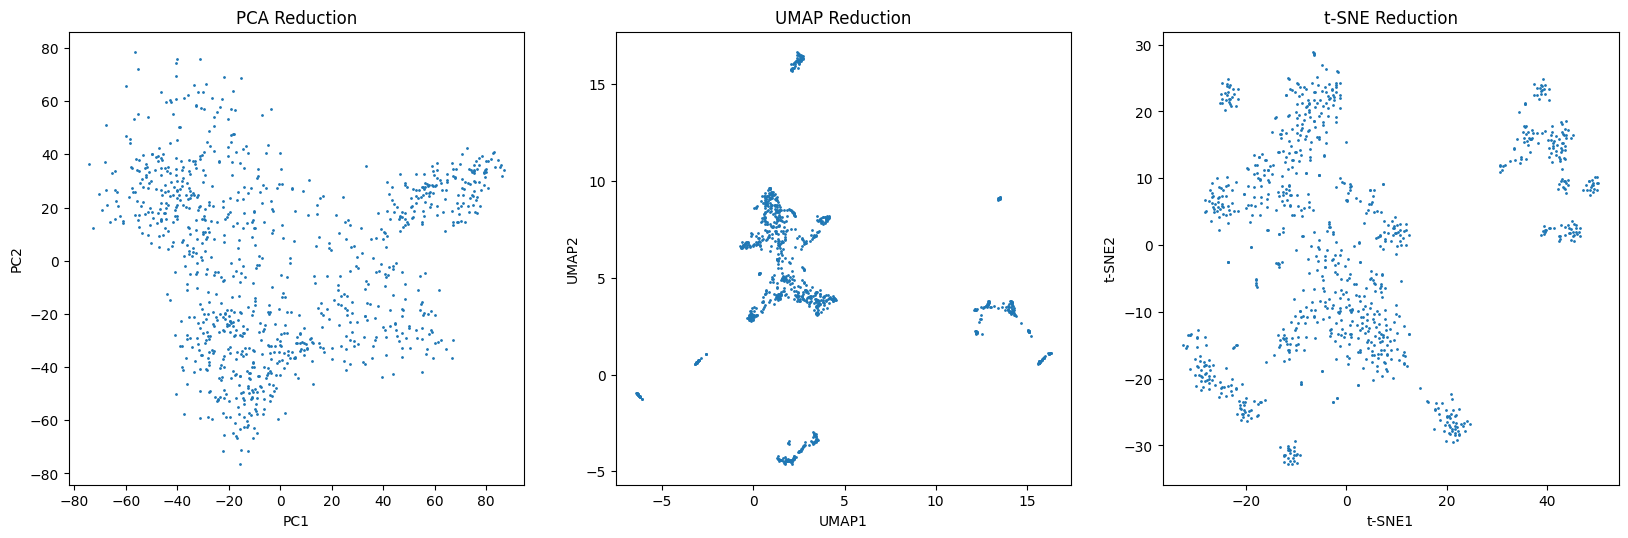
\includegraphics[width=\textwidth]{Images/default_dimred.png}
    \caption{PCA (left), UMAP (middle), and t-SNE (right) reduction using default parameters.}
    \label{fig:default_dimred}
\end{figure}

A quick implementation with the default parameters of each technique gives some insight into the nature of the performance. As seen in Figure \ref{fig:default_dimred}, distinct regions of point clusters have been generated in both the UMAP and t-SNE plots. The PCA plot, however, does not show any distinct clusters and instead shows a large cloud of points with no discernible structure. Knowing that both UMAP and t-SNE are non-linear techniques, it can be deduced that perhaps linear methods, such as PCA, are not the most suitable dimensionality reduction approaches for this dataset.

Another point to note is that while both UMAP and t-SNE have generated distinct clusters, the clusters are not identical in shape or density. UMAP has produced denser clusters that are closer to the origin, while t-SNE has produced a similar amount of clusters that are more spread out, both in terms of point-to-point and cluster-to-cluster. To examine the non-linear techniques further, parameters of interest were changed in isolation to analyze their effect on the resulting plots. 

\subsubsection{UMAP Parameter Analysis}
A sequence of reductions with varying number of neighbors in UMAP is observed in Figure \ref{fig:UMAP_vary}.

\begin{figure}[H]
    \centering
    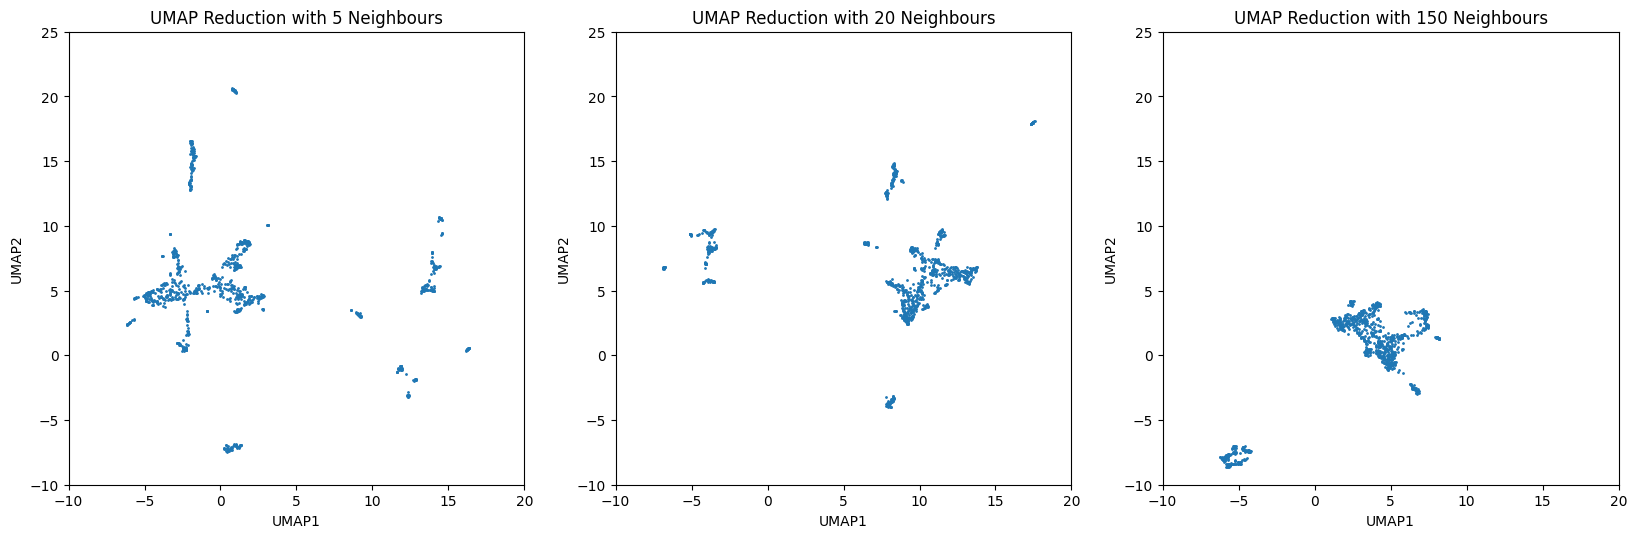
\includegraphics[width=\textwidth]{Images/UMAP_vary.png}
    \caption{UMAP reduction of the data varying the number of neighbors.}
    \label{fig:UMAP_vary}
\end{figure}

Visually, adjusting the number of neighbors considered in a UMAP reduction provides a different insight into the relationships between data points. As seen in Figure \ref{fig:UMAP_vary}, the number of clusters identified by the algorithm decreases as the number of neighbors increases. It can be discerned then, that considering more neighbors captures broader trends in the data, while considering fewer neighbors captures more local trends.

A sequence of reductions with varying minimum distance in UMAP is observed in Figure \ref{fig:UMAP_vary2}.

\begin{figure}[H]
    \centering
    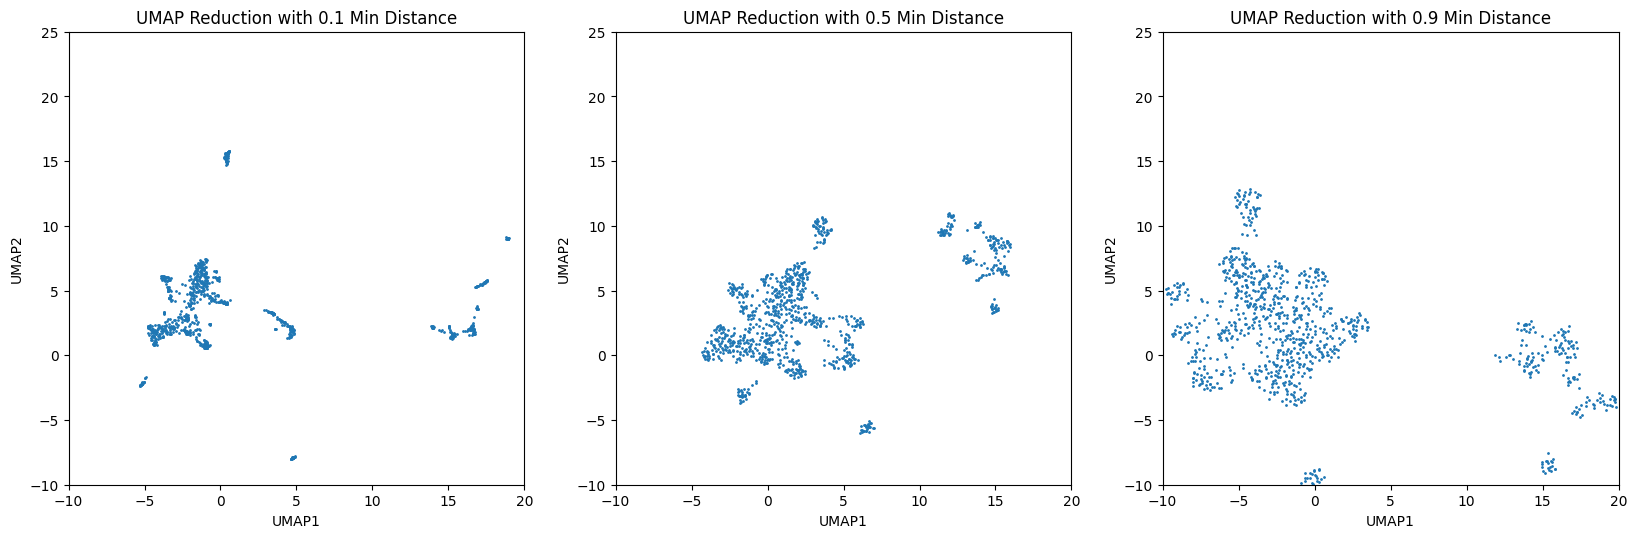
\includegraphics[width=\textwidth]{Images/UMAP_vary2.png}
    \caption{UMAP reduction of the data varying the minimum distance.}
    \label{fig:UMAP_vary2}
\end{figure}

From inspection, the minimum distance parameter seems to have a spread effect on the clusters and data points. As the minimum distance increased, the clusters reduced in number and became more spread out. This is likely due to the fact that the minimum distance parameter is used to control the effective minimum distance between points. As the minimum distance increases, the algorithm is forced to spread out the clusters to meet the minimum distance requirement.

Depending on the objective of the dimensionality reduction, both the number of neighbors and the minimum distance parameters can be used to control the generalization of the algorithm. If the goal is to identify broad trends in the data, then a higher number of neighbors and a lower minimum distance should be used. If the goal is to identify local trends in the data, then a lower number of neighbors and a higher minimum distance should be used.

\subsubsection{t-SNE Parameter Analysis}
A sequence of reductions with varying perplexity in t-SNE is observed in Figure \ref{fig:TSNE_vary}.

\begin{figure}[H]
    \centering
    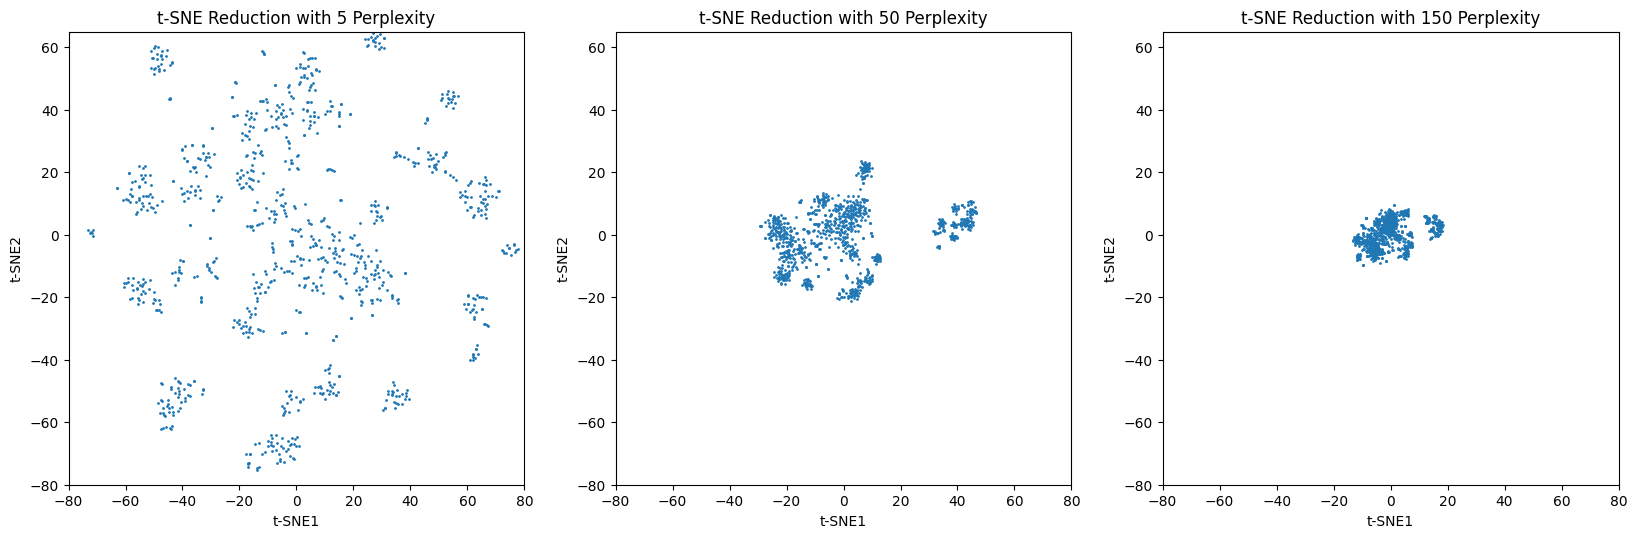
\includegraphics[width=\textwidth]{Images/t-sne_vary.png}
    \caption{t-SNE reduction of the data varying the perplexity.}
    \label{fig:TSNE_vary}
\end{figure}

Similar to the number of neighbors parameter in UMAP, the perplexity parameter in t-SNE controls the number of neighbors considered when reducing the dimensionality of the data. As seen in Figure \ref{fig:TSNE_vary}, the number of clusters identified by the algorithm decreases as the perplexity increases. It can be similarly discerned then that considering more neighbors captures broader trends in the data, while considering fewer neighbors captures more local trends.

Again, depending on the objective of the dimensionality reduction, the perplexity parameter can be used to control the generalization of the algorithm. If the goal is to identify broad trends in the data, then a higher perplexity should be used. If the goal is to identify local trends in the data, then a lower perplexity should be used.

\subsection{Discussion of Results}
\begin{enumerate}
    \item Do you see different clusters forming (visually)? How much correspondence exist
    between clusters that you find in different methods?
\end{enumerate}

\section{Part 2: Clustering}
\subsection{Agglomerative Clustering}
\subsubsection{Theory}

\subsubsection{Implementations}

\subsubsection{Results}

\subsection{K-Means Clustering}
\subsubsection{Theory}

\subsubsection{Implementation}

\subsubsection{Results}

\subsection{Comparison of Clustering Techniques}
\subsubsection{Jaccard Similarity}

\subsubsection{Rand Index}

\subsubsection{Adjusted Rand Index}

\newpage

\bibliographystyle{IEEEtran}
\bibliography{references}

\end{document}
